\documentclass[12pt]{article}

\usepackage[T2A]{fontenc}
\usepackage[utf8]{inputenc}
\usepackage[russian]{babel}
\usepackage[margin=0.5in]{geometry}
\usepackage{graphicx}
\usepackage{amsmath}
\usepackage{amsfonts}
\usepackage{indentfirst}
\usepackage{algorithm}
\usepackage{algpseudocode}

\graphicspath{{img/}}

%\setpapersize{A4}
%\setmarginsrb{30mm}{20mm}{20mm}{20mm}{0pt}{0mm}{0pt}{0mm}

\title{Модель навигации в транспортных сетях \\
       A model of navigation in transport networks}
\date{\vspace{-5ex}}
 
\begin{document}

\thispagestyle{empty}
\begin{center}

\includegraphics{msu.png}
\end{center}
\begingroup \fontsize{14pt}{16pt}\selectfont
\centerline{Московский
государственный
университет
имени М.В. Ломоносова}
\centerline{Факультет Вычислительной математики и кибернетики}
\centerline{Кафедра Алгоритмических Языков}
\vfill
\vfill
\vfill
\vfill
 \fontsize{22pt}{24pt}\selectfont
\centerline{Курсовая работа}
\vfill
 \fontsize{20pt}{24pt}\selectfont
\begin{center}
{\bf   Модель навигации в транспортных сетях}
\end{center}
\normalsize
\vfill
\vfill
\vfill
\vfill
\large
\begin{flushright}
\textbf{Выполнил:}

студент 325 группы

Бондарь Артём Александрович

\vfill
\textbf{Научный руководитель:}

к.ф.-м.н. доцент, учёный секретарь кафедры

Абрамов Владимир Геннадьевич
\end{flushright}
\normalsize
\vfill
\vfill
\vfill
\centerline{Москва~---            2018}
\endgroup

\pagebreak
\tableofcontents
\pagebreak

\section{Введение}

\subsection{Актуальность задачи}

В связи с растущим интересом к динамическому управлению транспортных систем, возникает необходимость находить кратчайшие пути в большом графе (например, дорожной сети), где вес или задержки, связанные с ребрами, динамически изменяются со временем. Появляются транспортные системы, которые могут обеспечивать в режиме реального времени данные о ситуации на дорогах. (например, VICS \cite{vics} или TMC \cite{tmc}). Совместно с доступностью топологий дорожных сетей и информации об движении на них, собранной за значительный промежуток времени, становится возможным использовать эти данные для предоставления лучших услуг по навигации в транспортных системах, учитывая закономерности движения внутри них.

\subsection{Предметная область}

Сферой исследования являются алгоритмы поиска крайтчайшего пути на графах, имитирующих траспортные системы. Из чего естественным образом можно вывести следующие свойства, присущие этим графам:

\begin{itemize}
  \item Ориентированность
  \item Неотрицательный вес рёбер
  \item Изменение топологии графа в течении времени
  \item Изменение весов рёбер графа в течении времени
  \item Изменения могут быть как случайными, так и запланированными
\end{itemize}

Таким образом, пользуясь классификацией, предложенной в обзоре существующих алгоритмов поиска кратчайшего пути \cite{survey}, выделим те типы алгоритмов, область примения которых ближе всего подходит к графам с вышеперечисленными свойствами. (см. рис. 1)

\begin{center}
  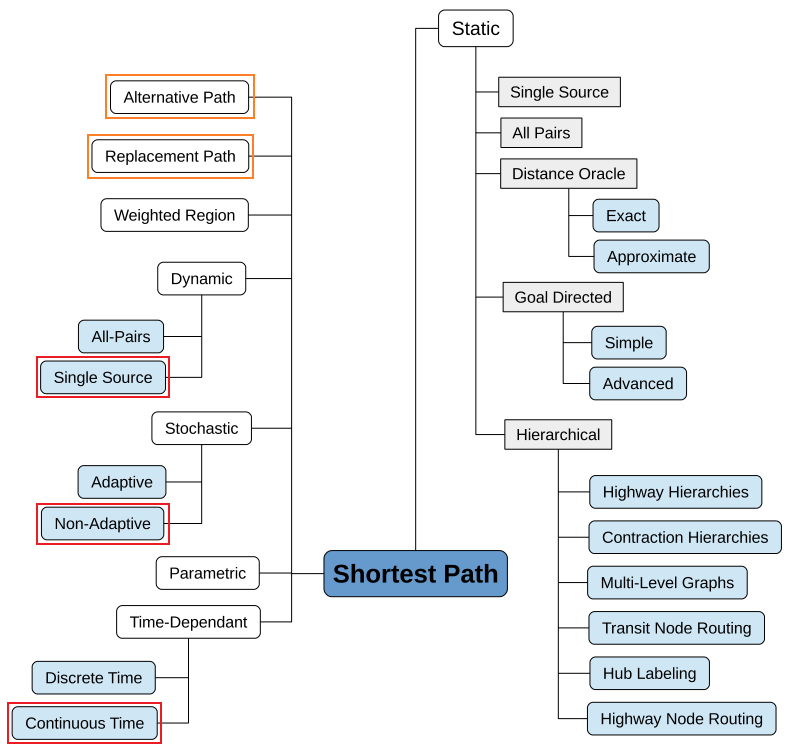
\includegraphics[scale=0.7]{taxonomy.png} \\
  Рис. 1
\end{center}

То есть, при поиске кратчайшего пути в дорожной сети мы гарантированно столкнёмся со следующими задачами:

\begin{enumerate}
  \item Поиск кратчайшего пути из одного источника в динамических графах. \\ \\
  Пусть задан граф $G = (V,E)$ с весами ребёр $f(e)$ и выделенной вершиной (называемой \textit{источником}) $u$. При этом множество вершин графа фиксировано, а множество ребёр может изменятся. Т.е. ребра могут произвольно быть удалены и/или добавлены. Последовательность $P(u,v)$ рёбер $e_1=(u,w_1), e_2=(w_1,w_2)$, …, $e_k=(w_{k-1},v)$ называется \textit{путём}, идущим от вершины $u$ к вершине $v$. Суммарный вес этого пути равен
  $$ f(P(u,v)) = \sum_{i = 1}^k f(e_i) $$  
  Требуется для каждой вершины $v$, достижимой из вершины-источника $u$, указать путь $P^*(u,v)$, имеющий наименьший суммарный вес:
  $$ f^*(v) = f(P^*(u,v)) = \min f(P(u,v)) $$
  
  \item Поиск кратчайшего пути в стохастических графах в условиях неопределённости. \\ \\
  
  Граф называется \textit{стохастическим}, если веса его ребёр представлены случайными величинами. \textit{Условиями неопределённости} следует считать состояние, при котором распределение случайных величин неизвестно.
  
  \item Поиск кратчайшего пути в графах с весами, задаваемыми функциями от непрерывного времени \\ \\
  Cчитая временной отрезок множеством $T$, пусть $T \in \mathbb{R}$ и $f: E \times T \rightarrow \mathbb{R}$. Тогда:
  
  $$ \lim_{t\to t_0} f(e,t) = f(e,t_0) $$
  
\end{enumerate}

Также, с большой вероятностью потребуется решать ещё две проблемы:

\begin{enumerate}
\setcounter{enumi}{3}
  \item Поиск кратчайшего альтернативного пути.
  
  Для пути $P(u,v)$, состоящем из рёбер $e_1, e_2, …, e_k$ \textit{альтернативным} называется такой путь $P^\prime(u,v)$, который не включает в себя ни одного ребра из множества рёбер $E^\prime= \{e_1, ..., e_k\}$.
  
  \item Поиск кратчайшего заменяющего пути.
  
  Путь $P^\prime(u,v)$ называется \textit{заменяющим} для пути $P(u,v)$, если не содержит ни одного ребра из множества $E^{\prime\prime}$, где $E^{\prime\prime} \subseteq E^\prime, |E^{\prime\prime}| \neq 0$
  
\end{enumerate}

Однако, это не означает, что задача строго укладывается в указанные рамки. Вполне возможно успешное применение наработок и с других областей, например, использование иерархических стуктур и/или каких-нибудь более эффективных форматов хранения и обработки информации о графах (или промежуточных вычислений).

\subsection{Сфера применения}

Наиболее востребованными алгоритмы поиска кратчайшего пути являются при использование в средствах навигации. Перечислим возможности, при наличии которых значительно возрастает эффективность практического использования:

\begin{itemize}
  \item Получение информации об изменениях в графе с различных источников в реальном времени
  \item Использование распределённых ресурсов (в том числе удалённых)
  \item Проведение предварительных вычислений там, где это возможно
  \item Поскольку все ещё не всегда и/или везде возможно иметь подключения к сети, требуется возможность работы автономно на устройствах с относительно малой вычислительной мощностью
  \item Быстрое просчитывание хотя бы начала пути, чтобы не тратить лишнее потенциальное время в дороге на ожидание результатов
  \item Просчитывание дальнейшего маршрута, поиск оптимальных альтернативных путей во время самого движения, а не только до него
\end{itemize}

Из перечисленных специфик следует почти полное отсутствие ограничений по памяти и сложности для предварительных вычислений и относительно не высокие требования к средней продолжительности вычислений, что позволяет частично уйти от вопросов оптимизации и сосредоточиться на точности полученных результатов.

\section{Обзор существующих решений}

\subsection{Базовые алгоритмы}

Классической тройкой алгоритмов, на базе которых строятся множество других различных алгоритмов поиска кратчайшего пути, являются:

\subsubsection{Алгоритм Дейкстры}

Дан взвешенный ориентированный граф $G(V,E)$ без дуг отрицательного веса. Алгоритм находит кратчайший путь от некоторой вершины $s$ графа $G$ до всех остальных вершин этого графа.

\begin{algorithm}
\caption{Dijkstra's algorithm}
\begin{algorithmic}[1]

\State \textbf{for} each vertex $v \in \id{V_G}$ \\
    \qquad $\at{dist}[v] \gets \infty$ \\
    \qquad $\at{parent}[v] \gets \const{NIL}$ \\
$\at{dist}[s] \gets 0$ \\
\\
$Q \gets \id{V_G}$
\State \textbf{while} $Q \neq \emptyset$ \\
\qquad $u \gets \text{Extract-Min}(Q)$ \\
\qquad \textbf{for} each edge $e = (u,v)$ \\
\qquad \qquad \textbf{if} $\at{dist}[v] > \at{dist}[u] + \at{weight}[e]$ \\
\qquad \qquad \qquad $\at{dist}[v] \gets \at{dist}[u] + \at{weight}[e]$ \\
\qquad \qquad \qquad $\at{parent}[v] \gets u$ \\
\\
$H \gets (\id{V_G, \emptyset})$
\State \textbf{for} each vertex $v \in \id{V_G},\ v \neq s$ \\
    \qquad $\id{E_H} \gets \id{E_H} \cup \{(\at{parent}[v], v)\}$ \\
\Return $H, \id{dist}$
\end{algorithmic}
\end{algorithm}

На стадии инициализации каждой вершине, кроме начальной $s$, присваивается метка бесконечности и нулевой путь, начальной же вершине полагается метка 0. (строки 1-4)

Пока все вершины не были пройдены, из ещё не посещённых вершин выбирается вершина $u$, имеющая минимальную метку. Для каждого соседа вершины $u$, кроме отмеченных как посещённые, рассмотрим новую длину пути, равную сумме значений текущей метки $u$ и длины ребра, соединяющего $u$ с этим соседом. Если полученное значение длины меньше значения метки соседа, заменим значение метки полученным значением длины. Рассмотрев всех соседей, пометим вершину $u$ как посещённую и повторим шаг алгоритма. (строки 6-12)

Далее остаётся только собрать полученные пути и вернуть результат. (строки 14-18)

\subsubsection{Алгоритм Беллмана-Форда}

Дан ориентированный или неориентированный граф $G$ со взвешенными рёбрам без отрицательных циклов. Требуется найти кратчайшие пути от выделенной вершины $s$ до всех вершин графа. Цикл, сумма весов рёбер которого отрицательна, называется \textit{отрицательным циклом}.

\begin{algorithm}
\caption{Bellman–Ford algorithm}
\begin{algorithmic}[1]

\State \textbf{for} $v \in \id V$ \\
    \qquad $\at{dist}[v] \gets +\infty$ \\
    \qquad $\at{parent}[v] \gets \const{NIL}$ \\
$\at{dist}[s] \gets 0$ \\

\State \textbf{for} $i \gets 1$ \textbf{to} $|V|-1$ \\
\qquad \textbf{for} $(u,v) \in E$ \\
\qquad \qquad \textbf{if} $\at{dist}[v] > \at{dist}[u] + \at{weight}(u,v)$ \\
\qquad \qquad \qquad $\at{dist}[v] \gets \at{dist}[u] + \at{weight}(u,v)$ \\
\qquad \qquad \qquad $\at{parent}[v] \gets u$ \\
\Return $dist$
\end{algorithmic}
\end{algorithm}

Используется те же метки, что и в алгоритме Дейкстры, инициализация аналогична. Разница в том, что вместо обхода вершин рассматриваются все возможные пути из $s$, длина которых не более $i$ рёбер.

\subsubsection{А*}

Дан взвешенный граф $G$. Алгоритм ищет маршрут наименьшей стоимости от выбранной начальной вершины $s$ до выбранной конечной $d$. В процессе работы для вершин рассчитывается функция $f(v)=g(v)+h(v)$, где

\begin{itemize}
    \item $g(v)$ — наименьшая стоимость пути в $v$ из стартовой вершины
    \item $h(v)$ — эвристическое приближение стоимости пути от $v$ до конечной цели
\end{itemize}

%\vfill

\begin{algorithm}
\caption{A* search algorithm}
\begin{algorithmic}[1]

\State open $\gets s$ \\
close $= \oslash$ \\
$g[s]=0$ \\
$f[s]=g[s]+h[s]$
\\
\State \textbf{while} close $\neq 0$ \\
\qquad {$x = \min\limits_{f(x)} \in $} open \\
\qquad \textbf{if} $x = d$ \\
\qquad \qquad \textbf{return} $true$ \\
\qquad open $\rightarrow x$ \\
\qquad close $\gets x$ \\
\qquad \textbf{for} $v \in neighbours(x)$ \\
\qquad \qquad cost $= g[x] + weight(x, v)$ \\
\qquad \qquad \textbf{if} $v \in $ close \textbf{and} cost $\beq g[v]$ \\
\qquad \qquad \qquad \textbf{continue} \\
\qquad \qquad \textbf{if} $v \notin $ close \textbf{or} cost $< g[v]$ \\
\qquad \qquad \qquad $parent[v] = x$ \\
\qquad \qquad \qquad $g[v] = $ cost \\
\qquad \qquad \qquad $f[v] = g[v] + h[v]$ \\
\qquad \qquad \qquad \textbf{if} $v \notin $ open \\
\qquad \qquad \qquad \qquad open $\gets v$ \\

\Return $false$
\end{algorithmic}
\end{algorithm}

%\pagebreak

Обозначения:

\begin{itemize}
    \item open — множество вершин, которые требуется рассмотреть
    \item close — множество рассмотренных вершин
    \item $f[x]$ — значение эвристической функции "расстояние + стоимость" для вершины $x$
    \item $g[x]$ — стоимость пути от начальной вершины до $x$
    \item $h(x)$ — эвристическая оценка расстояния от вершины x до конечной вершины.
\end{itemize}

На каждом этапе работы алгоритма из множества open выбирается вершина с наименьшим значением эвристической функции и просматриваются её соседи. Для каждого из соседей обновлятся расстояние, значение эвристическо функции и он добавляется в множество open. Поведение алгоритма сильно зависит от того, какая эвристика используется. В свою очередь, выбор эвристики зависит от постановки задачи.
 
\subsubsection{Сложность алгоритмов}

Худшую вычислительную сложность имеет алгоритм Беллмана-Форда - $O(|V||E|)$, зато у него самое широкое применение. Немного лучше сложность у алгоритма Дейкстры - $O(|V|^2)$. \\
Временная сложность алгоритма A* зависит от эвристики. В худшем случае, число вершин, исследуемых алгоритмом, растёт экспоненциально по сравнению с длиной оптимального пути, но сложность становится полиномиальной, когда эвристика удовлетворяет следующему условию:

$$|h(x)-h^*(x)| \leq O(\log h^*(x))$$, где $h^*$ — оптимальная эвристика, то есть точная оценка расстояния из вершины $x$ к цели. 

Таким образом, в своем изначальном варианте эти алгоритмы плохо применимы для больших динамических транспортных графов с переменными значениями рёбер. Первые два - в силу большой вычислительной сложности, а последний - в виду сложности выбора эвристики приближенной к оптимальной.

\subsection{Модификации базовых алгоритмов}

\subsubsection{2S-LTT}

Двухшаговый алгоритм \cite{2s-ltt}, основанный на алгоритме Дейкстры, для графов большой размерности с весами рёбер, задаваемыми функцией от времени. При этом также начальным параметром является временной интервал - промежуток времени, в который можно выехать из пункта отправления.

\begin{algorithm}
\caption{Two-Step-LTT$(G_T(V,E,W),v_s,v_e,T)$}
\textbf{Input:} a time-dependent graph $G_T$, a query LTT$(v_s,v_e,T)$ - \\
source $v_s$, destination $v_e$, and starting-time interval $T = [t_s,t_e];$ \\
\textbf{Output:} optimal $v_s-v_e$ path $p^*$, and optimal starting time $t^*$. \\
\begin{algorithmic}[1]
\State $\{g_i(t)\} \gets timeRefinement(G_t,v_s,v_e,T);$ \\
\textbf{if} $\neg (g_e(t) = \infty $ for the entire $[t_s,t_e])$ \textbf{then} \\
\qquad $t^* \gets$ arg$\min_{t \in T} \{g_e(t)-t\};$ \\
\qquad $p^* \gets pathSelection(G_T, \{g_i(t)\},v_s,v_e,t^*);$ \\
\qquad \textbf{return} $(t^*,p^*);$ \\
\textbf{else return} $\emptyset$
\end{algorithmic}
\end{algorithm}

Вычисления проходят в две фазы, на первом шаге вычисляется самое быстрое время прибытия для каждого ребра, на втором происходит выбор пути. Фактически, от алгоритма Дейкстры 2S-LTT отличается только первым шагом, поскольку выбор пути происходит аналогично:

\begin{algorithm}
\caption{$pathSelection(G_T(V,E,W), \{g_i(t)\},v_s,v_e,t^*);$}
\textbf{Input:} a time-dependent graph $G_T$, the set of earliest arrival-time \\
functions $g_i(t)$  for all nodes $v_i \in V$, source node $v_s$, destination \\
node $v_e$, and the optimal starting time $t^*;$ \\
\textbf{Output:} an optimal $v_s-v_e$ path $p^*$ for starting time $t^*$. \\
\begin{algorithmic}[1]
\State $v_j \gets v_e;$ \\
$p^* \gets \oslash;$ \\
\textbf{while} $v_j \neq v_s$ \textbf{do} \\
\qquad \textbf{for each} $(v_i,v_j) \in E$ \textbf{do} \\
\qquad \qquad \textbf{if} $g_i(t^*) + w_{i,j}(g_i(t^*)) = g_j(t^*)$ \textbf{then} \\
\qquad \qquad \qquad $v_j \gets v_i;$ \textbf{break;}\\
\qquad $p^* \gets (v_i,v_j)\cdot p^*$ \\
\textbf{return} $p^*$
\end{algorithmic}
\end{algorithm}

Алгоритм ищет наименьшее время прибытия с условием возможности ожидания на вершинах. Полученная вычислительная сложность: $O((|V|\log|V|+|E|)\alpha(T))$, где $\alpha(T)$ - стоимость применимых функций. 

\subsubsection{OR}

Относительно простым алгоритмом является обобщение алгоритма Беллмана-Форда - OR \cite{or} (назван по первым буквам инициалов авторов).

\begin{algorithm}
\caption{Bellman-Ford Based Algorithm}
\begin{algorithmic}[1]
\State \textbf{for all} $v_t \in V$ \textbf{do} $g_t(t) \gets \inf$ for $t \in T;$
\State \textbf{for all} $(v_k,v_l) \in E$ \textbf{do} $h_{k,l}(t) \gets \inf$ for $t \in T;$
\State $g_s(t) \gets t$ for $t \in T;$
\Repeat
\State \textbf{for all} $(v_k,v_l) \in E$ \textbf{do} $h_{k,l}(t) \gets g_k(t) + w_{k,l}(g_k(t));$
\State \textbf{for all} $v_l \gets V$ \textbf{do} $g_l(t) \gets \min_{v_k \in N(v_l)}\{h_{k,l}(t)\};$
\Until all functions $g_l(t)$ are unchanged \\
\Return $(t^* \gets$ arg$\min_{t \in T} \{g_e(t) - t\},p^*);$
\end{algorithmic}
\end{algorithm}

Пусть $g_l(t)$ - время кратчайшего прибытия в вершину $v_l$ из вершины $v_s$ за начальное время $t$ и пусть
$h_{k,l}(t)$ - кратчайшее время прибытия в $v_l$ из $v_s$ за время $t$ через ребро $(v_k,v_l)$. \\
Сначала инициализируются функции $g_l(t)$ и $h_{k,l}(t)$  (строки 1-3), а потом происходит повторяющиеся обновления $g_l(t)$ и $h_{k,l}(t)$ до тех пор, пока они не сойдутся до правильных значений (строки 4-7). \\
Наконец (строка 8), происходит возрат лучшего начального времени $t^*$ и оптимального пути $p^*$, который высчитывается на основе $g_l(t)$ и $h_{k,l}(t)$. 

Временная сложность алгоритма - $O(|V||E|\alpha(T))$, что делает его не применимым для больших временных графов. 


\subsubsection{KDXZ}

Данный алгоритм \cite{kdxz}, тоже названный по первым буквам инициалов авторов, является расширением A* алгоритма на случай графов с весами, зависящими от времени. Главная идея схожа - происходит обработка очереди $Q$ всех возможных путей. Пускай $p_k$ - это путь от начальной вершины $v_s$ к вершине $v_k$ в графе $G_T$. Возможно существование нескольких путей из $v_s$ в $v_k$ и все из них будут содержаться в $Q$ одновременно. Для каждого пути $v_k$ высчитывается функция $f_{p_k}(t)=g_{p_k}(t)+d_{k,e}-t$, где:
\begin{itemize}
    \item $g_{p_k}(t)$ - время прибытия из $v_s$ в $v_k$ начиная с времени $t$
    \item $d_{k,e}$ - эвристическая функция, представляющая собой нижнюю оценку предполагаемой продолжительности пути из $v_k$ в конечную вершину $v_e$
    \item $f_{p_k}(t$ - оценочное время пути из $v_s$ в $v_e$ по пути $p_k$ с начального момента времени $t$
\end{itemize}

На каждой итерации, выбирается путь $p_i \in Q$, такой, что $\min_{t}\{f_{p_i}(t)\} = \min\limits_{p_k \in Q}_t\{f_{p_k}(t)\}$  $\forall k$ \\
Каждый путь $p_j$, получаемый увеличением путя $p_i$ на одно ребро $(v_i,v_j)$ добавляется в очередь $Q$, а путь $p_i$ удаляется. Процесс остановится, когда будет получен первый путь $v_s-v_e$.

Алгоритм KDXZ эффективен только тогда, когда выбранная эвристика эффективно сокращает ширину поиска, а $v_s$ и $v_e$ относительно близко расположены друг к другу. К тому же выбор эвристики $d_{k,e}$ для обобщённых графов достаточно сложен. В худших случаях, при удалённых на значительное расстояние начальной и конечной вершинах и/или выборе не оптимальной эвристики получаемая сложность алгоритма экспоненциальна.

\subsubsection{Сравнение алгоритмов}

\begin{center}
  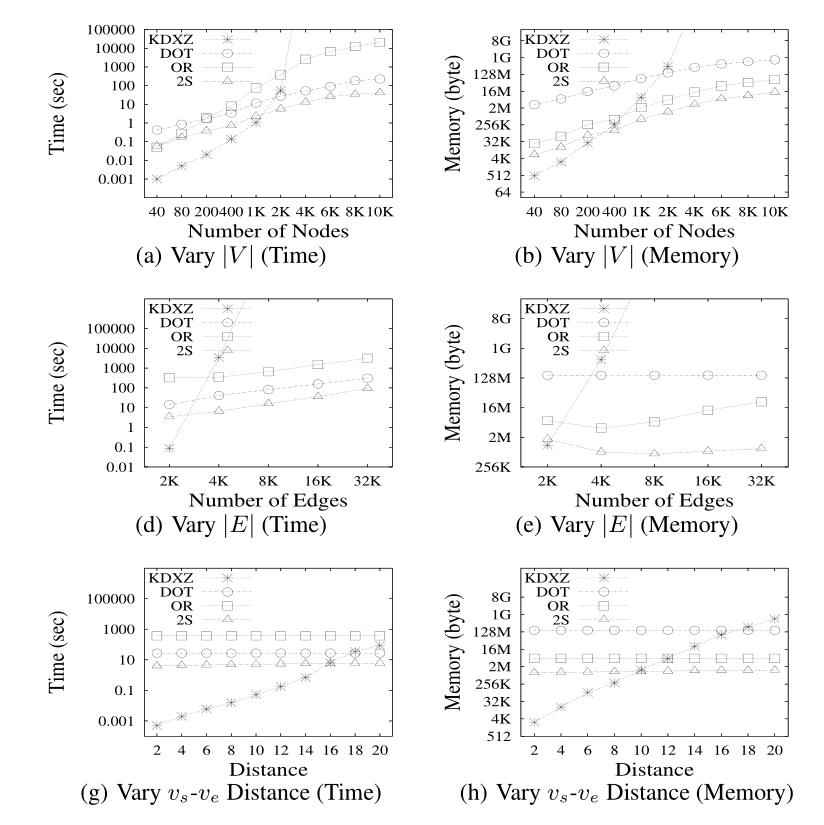
\includegraphics[scale=0.65]{comparing.png} \\
  Рис. 2
\end{center}

На Рис. 2 представлены результаты работы трёх предыдущих алгоритмов и ещё одного четвёртого - DOT \cite{dot}, который не был рассмотрен в виду того, что не попадает в исследуемую сферу алгоритмов (поскольку используется для графов с дискретным временем, а не непрерывным). 

Тестирование проводилось на 2.8GHz CPU с 1G RAM. В качестве основы для данных использовалась дорожная сеть штата Мэрилэнд в США, полученная системой TIGER/Line \cite{tiger}. Количество вершин - 16,326, рёбер - 26,528. Весы вершин были сгенерированы в случайном диапазоне. 

\subsection{Выводы}

Используя за основу классические алгоритмы, можно добиться довольно неплохих результатов при их расширении на временные графы, по крайней мере небольшого размера. При должной степени оптимизации вычислений, а также используя более продвинутые методики хранения и работы с данными, применяя различные подходы из других областей алгоритмов кратчайших путей (например, используя иерархические структуры) можно получить более эффективные реализации алгоритмов. 

Однако, глобальная проблема состоит в том, что существует зазор между теоретическим моделированием и реальной ситуацией. В транспортных системах происходит большое количество случайных событий (аварии, перекрытия дорог, снижение/увеличение плотности движения), которые нельзя заранее спрогнозировать (начиная от самого факта появления события и заканчивая конкретной величиной изменений). Из-за этого сильно падает точность вычислений, появляется необходимость учитывать динамику и распределение переменных величин.

Помимо этого, заранее вычисленные маршруты движения могут перестать быть минимальными по выбранному параметру вследствии поведения пользователя. Почти все теоретические алгоритмы принимают за аксиому, что будет произведено движение с определённой скоростью по определённому маршруту. Но в реальной жизни могут произойти отклонения, связанные с человеческим фактором, например, водитель может намеренно свернуть с оптимального пути по какой-то причине, может немного задержаться или просто снизить скорость движения.  

Проанализировав особенности транспортных систем и сферы использования можно прийти к выводу, что ни один из существующих алгоритмов в полной мере не удовлетворяет накладываемым ограничениям и требованиям к результатам в связи с тем, что эти ограничения и требования могут произвольно менятся. Следовательно, в связи с отсутствием теоретических решений, придётся применить экспериментальные прикладные методы.

\section{Постановка задачи}

\subsection{Параметры графа}

Задан ориентированный граф $G_T=(V,E)$, $V = \{v_i\}$ - множество вершин графа, $E \subseteq V \times V$ - множество рёбер, $T$ - область времени.
\begin{itemize}
    \item $t_0$ - начальное время
    \item $t_{cur}$ - текущее время
    \item $s$ - вершина, с которой началось движение
    \item $d$ - вершина, по направлению к которой происходит движение
    \item $l(e)$ - длина ребра, не меняется
    \item $A(e,t)$ - доступность ребра
\[
  A(e,t) =
  \begin{cases}
    1, & \text{если ребро $e(u,v)$ существует и доступно для прохождения} \\
    0, & \text{если ребро $e(u,v)$ не существует или запрещено для прохождения} \\
  \end{cases}
\]
    \item $T_{act}$ - интервал времени, на протяжении которого полученные данные считаются актуальными
    \item $v_{avg}(e,t)$ - средняя скорость движения на ребре $e(u,v)$ в момент времени $t=t_0$
    \item $v_{rec}(e)$ - средняя скорость движения на ребре $e(u,v)$ для последнего обновления
    \item $t_{rec}(e)$ - время последнего обновления средней скорости на ребре $e(u,v)$, инициализируется так:
\[
  \begin{cases}
    $$v_{rec}(e) = v_{avg}(e,t_0)$$ \\
    $$t_{rec}(e) = t_0$$
  \end{cases}
\]
    \item $v_{act}(e, t_0)$ - скорость движения на ребре $e(u,v)$, применяемая для вычислений в момент времени $t_0 > t_{cur}$
\[
  v_{act} =
  \begin{cases}
    $$v_{rec},$$ & \text{$t_{cur} - t_0 \leq T_{act}$} \\
    $$v_{avg},$$ & \text{$t_{cur} - t_0 > T_{act}$} \\
  \end{cases}
\]
    \item $\frac{l(e)}{v_{act}(e,t_0)}$ - вычисляемый вес ребра $e(u,v)$ в момент времени $t_0$

\end{itemize}

Последовательность $P(s,d)$ рёбер $e_1=(s,v_1), e_2=(v_1,v_2)$, …, $e_k=(v_{k-1},d)$ называется \textit{путём}, идущим от вершины $s$ к вершине $d$, причём $A(e_i,t_i)=1$ $\forall i$, где $t_i$ - момент попадания в начало ребра $e_i$.

Изменение времени задается рекурсивно:
$$t_i = t_{i-1} + \frac{l(e_i)}{v_{act}(e_i,t_i)}$$

Суммарная длительность пути равна:
$$L_t(P(u,v)) = \sum_{i = 1}^k \frac{l(e_i)}{v_{act}(e_i,t_i)}$$

Требуется для двух указанных вершин $s$ и $d$ привести такой путь $P(s,d)$, чтобы суммарная длительность были минимальными.

\subsection{Данные для приёма и передачи}

В любой момент времени $t_{cur}$ могут поступить следующие данные: \\
\{$u,v,v_{rec}$\} - обновление средней скорости на ребре $e(u,v)$, при получении $t_{rec}(e) = t_{cur}$ \\
\{$u,v,A(e(u,v),t),t_0,t_1$\} - доступность ребра $e(u,v)$ в интервале времени $[t_0,t_1]$ \\

Для вычислений передаются:
\{$G_T,t_0,A(e_i,t),T_{act},s,d,v_{avg}(e_i,t),v_{rec}(e_i),t_{rec}(e_i)$\} - слепок всех данных, используемых для вычислений кратчайшего пути, в момент времени $t_0$

Получаемые результаты вычислений:
\{$t_0,P,L_t$\}

\section{Модель навигации}

\subsection{Предпосылки}

В силу быстро растущей сложности просчитывания кратчайшего пути для динамического графа со случайными изменениями - это не является осуществимой в удобоваримый срок задачей даже для графов средней величины. Из-за случайного изменения параметров графа и непредсказуемого поведения \textit{выполняющего} алгоритм (например, водителя) становится бессмысленным просчитывание оптимального маршрута только единожды до выезда из отправной точки. Более того, просчёт второй половины пути может не пригодится, если что-то случится раньше того, как \textit{выполняющий} доберётся туда.

Таким образом, необходимо отслеживать в реальном времени все те события, которые могут поменять уже вычисленный результат и при их возникновении проводить перерасчёт кратчайшего пути. Для решения поставленной задачи предлагается реализация системы по управлению вычислениями, позволяющей производить:

\begin{itemize}
    \item Версионное хранение информации о состоянии графа - требуется для анализа полученных результатов, вычисленных на основе данных о уже возможно устаревшем графе
    \item Обработку поступающих изменений графа - правильно разбирать и сохранять данные об изменении топологии и средних скоростей на рёбрах, определять которые из них могут повлиять на корректность уже полученного результата
    \item Асинхронное оперирование различным количеством вычислительных узлов - организация приёма и передачи данных, эффективного использования ресурсов
    \item Анализ поступающих результатов вычислений - требуется определять по полученным результатам вносимые в текущий маршрут изменения, если таковые необходимы для уменьшения времени маршрута
    \item Корректирование работы в связи с изменениями параметров движения, зависящих от выбора выполняющего алгоритм - отслеживать в реальном времени, насколько точно происходит следование маршрута и в случае критических изменений срочно предпринимать меры по просчёту нового пути
\end{itemize}

В виду высокой сложности данной системы, она выходит за рамки курсовой работы. Поэтому в данной работе будет подробно рассмотрен только её отдельный компонент - сам алгоритм вычисления кратчайшего пути. Вообще говоря, сама система вычислений полностью независима от используемых в ней алгоритмов поиска кратчайшего пути, она оперирует только с передачей им параметров и возвращаемыми результатами, однако поскольку не существует подходящего алгоритма для работы с графами, предполагаемыми в задаче, все равно придётся реализовывать свою версию такого алгоритма. 

\subsection{Идея алгоритма}

Рассматривая проблему глобально, причина роста сложности напрямую зависит от количества вершин и ребёр в графе. С маленькими графами успешно может справится любой алгоритм за приемлимое время работы. Поскольку для нашей задачи подсчёт сразу всего пути бессмысленный, логично разбить весь путь на небольшие участки, на которых можно быстро подсчитывать кратчайший путь. Также, следует как можно сильнее ограничить уже разбитые участки, так чтобы не проводить лишних вычислений маршрутов через те зоны графа, которые очевидно лежат в стороне или вообще в противоположном направлении от вершины конца. Таким образом, рассматривая только небольшой подграф на нём можно добиться быстрого вычисления кратчайшего пути до его границы. Следует заметить, что этот же самый подход используется в алгоритмах, проводящих вычисления для графов с иерархией.

\pagebreak

Очевидной идеей для достижения пункта назначения является предпринятие движения в сторону этого самого пункта. Попробуем применить её для редуцирования графа. Допустим, у нас имеется некая дорожная сеть, граф которой изображём на Рис. 3а и нам необходимо попасть из вершины $s$ в вершину $d$. Проведём прямую между этими вершинами и выделим вокруг неё некоторую окрестность фиксированого радиуса $r$ от каждой точки прямой (в результате получится овальная область, как на Рис. 3б). Далее убираем все вершины, не попавшие в эту область и все рёбра, выходящие из них (результат показан на Рис. 3в). В итоге получим подграф с меньшим количеством вершин и рёбер. Помимо этого также можно убрать и все вершины, не состоящие в одном компоненте связности с вершинами $s$ и $d$. 

При достаточно большой длине $r$ большая часть кратчайших путей может попадать в область редуцирования. Рассмотрим возникающие при этом проблемы.

\begin{figure}
\minipage{0.33\textwidth}
  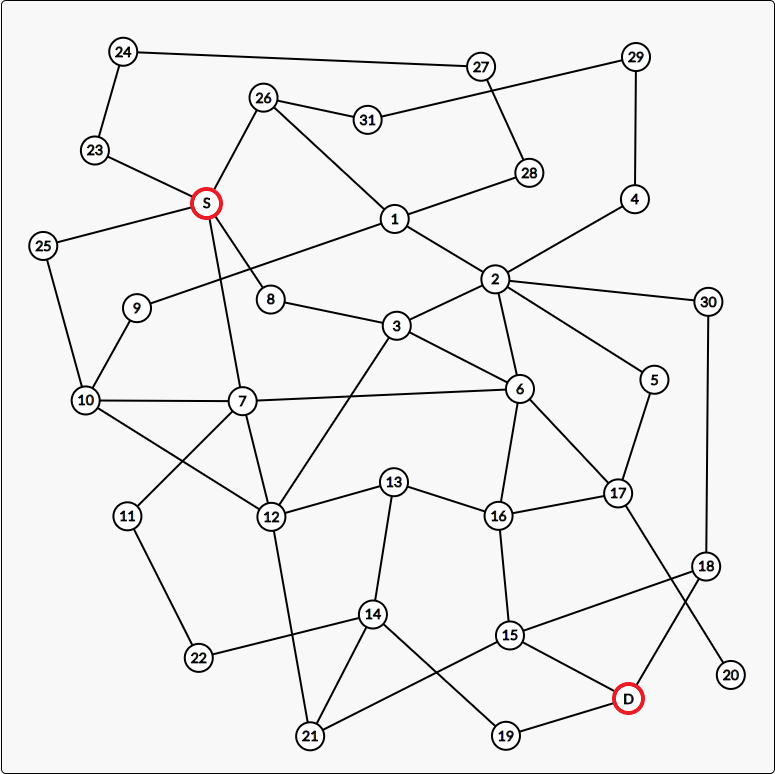
\includegraphics[width=\linewidth]{idea_01.png}
    \begin{center}
        Рис. 3а
    \end{center}
\endminipage\hfill
\minipage{0.33\textwidth}
  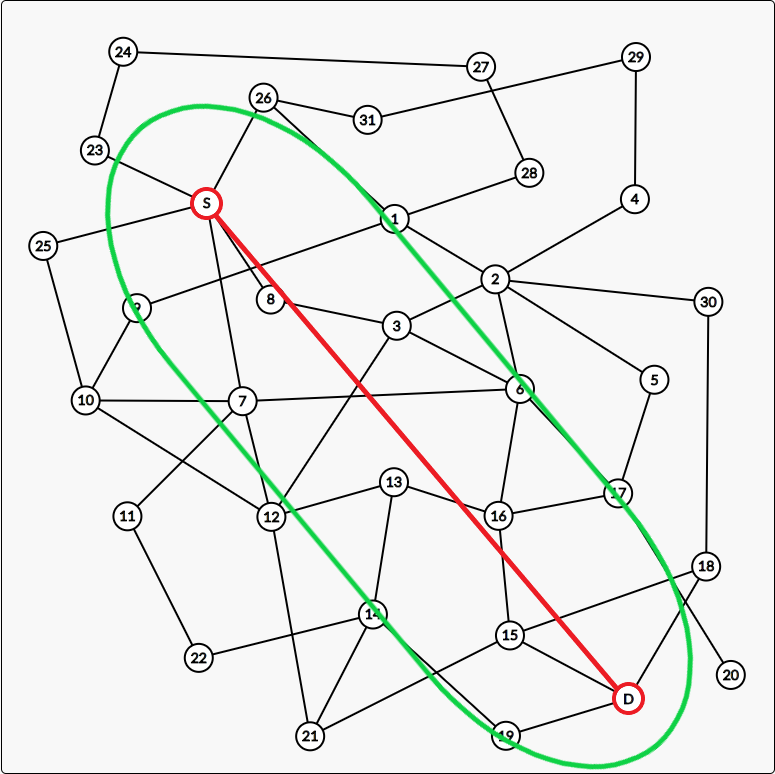
\includegraphics[width=\linewidth]{idea_02.png}
        \begin{center}
        Рис. 3б
    \end{center}
\endminipage\hfill
\minipage{0.33\textwidth}
  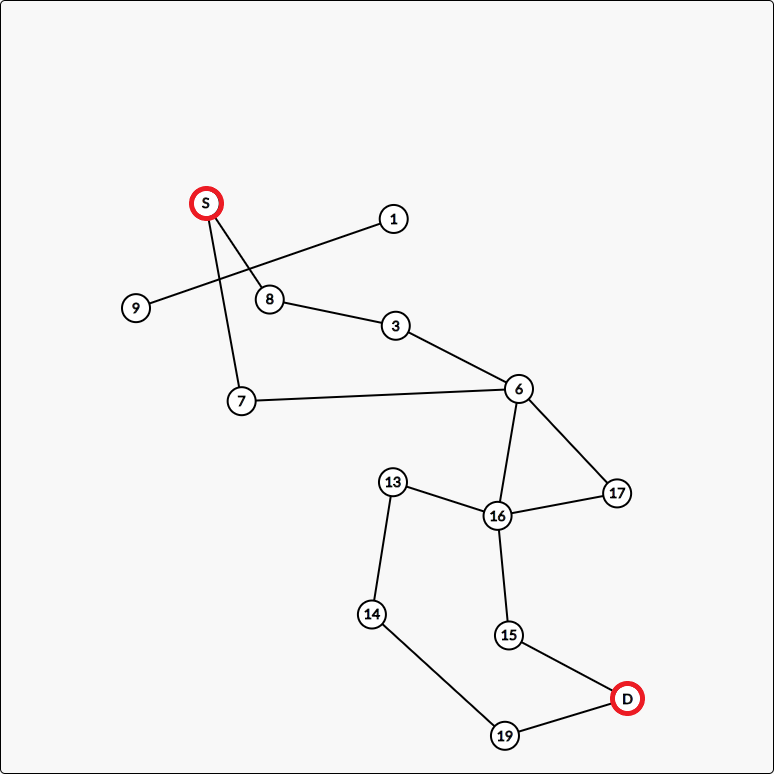
\includegraphics[width=\linewidth]{idea_03.png}
    \begin{center}
        Рис. 3в
    \end{center}
\endminipage
\end{figure}

\begin{enumerate}
    \item Существует некий окружной путь, не попавший в область редуцирования, однако при этом являющийся кратчайшим путём. Например, это может быть некая магистраль с повышенной скоростью движения (см. Рис. 4а)
    \item В области редуцирования отсутсвует путь из $s$ в $d$ и для его получения возможно придётся слишком сильно расширять эту область. (см. Рис. 4б)
    \item В области редуцирования находится подграф, не имеющий связи с вершиной концом, вследствии чего попадание в этот подграф будет напрасной тратой времени. (см. Рис. 4в)
\end{enumerate}

При этом отсуствие самого лучшего пути не является сильно критическим фактором, а вот остальные две проблемы делают данный подход не дееспособным. Поэтому необходимо как-нибудь иначе выбирать исходное направление к концу маршрута. Тут на помощь приходят обычные алгоритмы поиска кратчайшего пути. Рассмотрим следующую эвристическую гипотезу:
\\[0.5cm]
\textbf{Гипотеза.} Кратчайший путь \textit{по времени} находится недалеко от кратчайшего пути \textit{по расстоянию}.
\\[0.5cm]

\begin{figure}
\minipage{0.33\textwidth}
  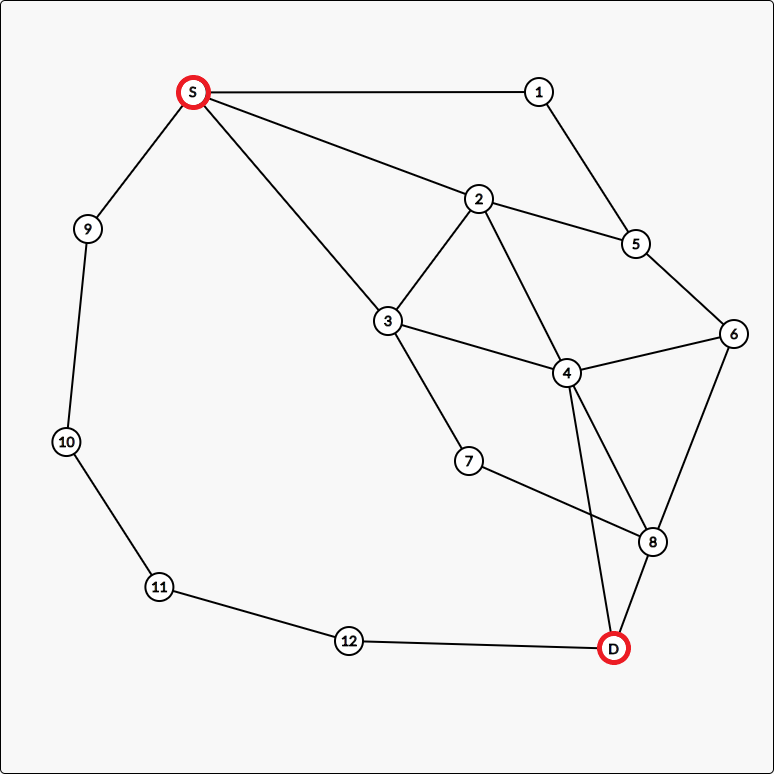
\includegraphics[width=\linewidth]{problem_01.png}
    \begin{center}
        Рис. 4а
    \end{center}
\endminipage\hfill
\minipage{0.33\textwidth}
  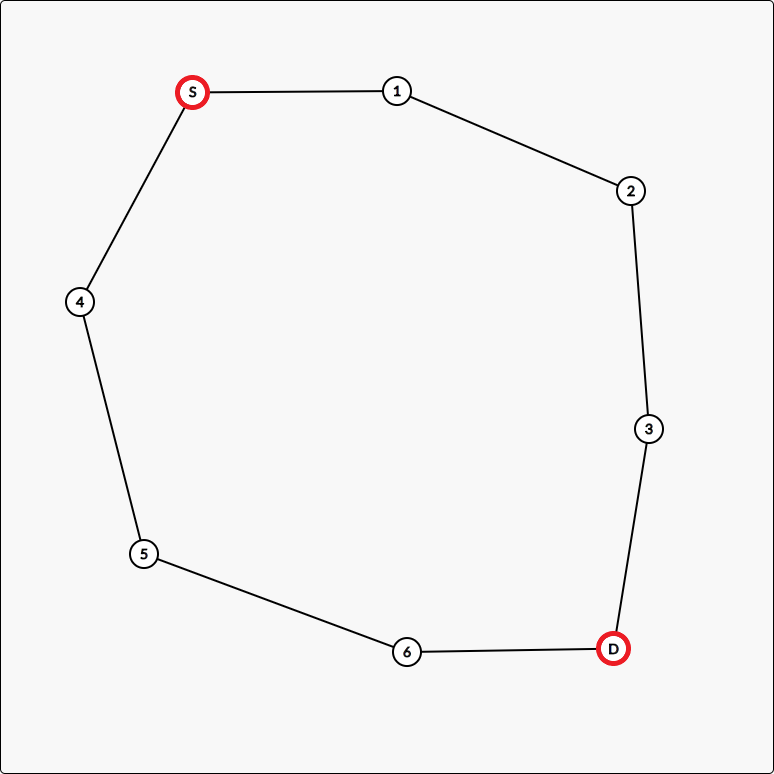
\includegraphics[width=\linewidth]{problem_02.png}
        \begin{center}
        Рис. 4б
    \end{center}
\endminipage\hfill
\minipage{0.33\textwidth}
  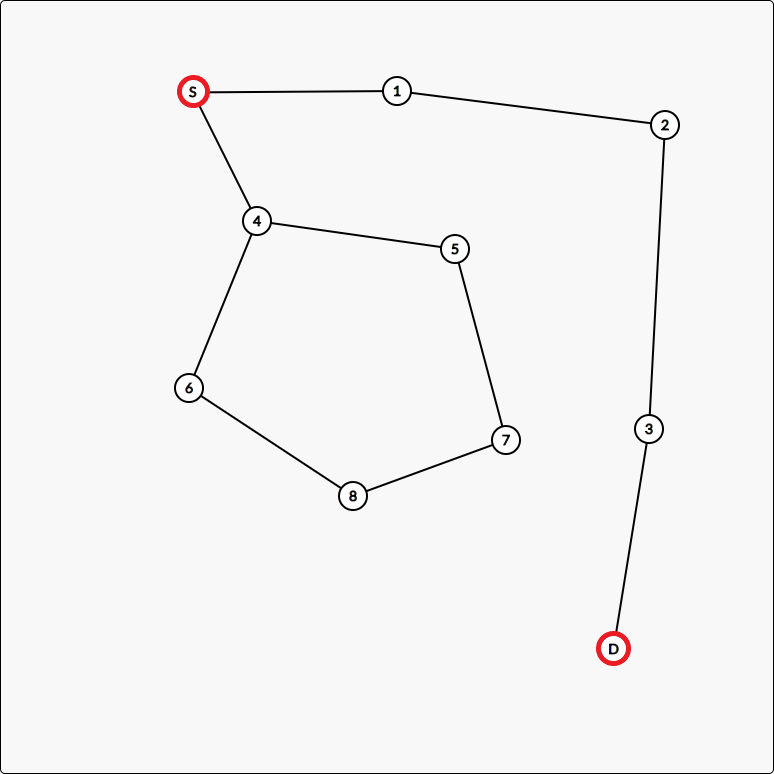
\includegraphics[width=\linewidth]{problem_03.png}
    \begin{center}
        Рис. 4в
    \end{center}
\endminipage
\end{figure}

Действительно, примем во внимание сильно разветлённые топологии городов, как самых часто используемых для навигации. Какие факты из этого следуют?

\begin{itemize}
    \item Наличие большого количества объездных дорог
    \item Очень маловероятен случай ухудшения движения в целом районе, чтобы его нельзя было объехать по соседним улицам
    \item Скоростные дороги имеют периодические заезды и выезды
\end{itemize}

Приведённые факты позволяют опустить проблему 1), поскольку если более короткий путь и будет пропущен, то в дальнейшем он сможет быть найден при вычислениях на больших областях. Проблемы 2) и 3) решаются автоматически. Решим последнюю существенную проблему, которая может возникнут при использовании такого способа выбора направления, а именно - проблема \textit{узких мест}. Рассмотрим топологию, изображённую на Рис. 5.

\begin{center}
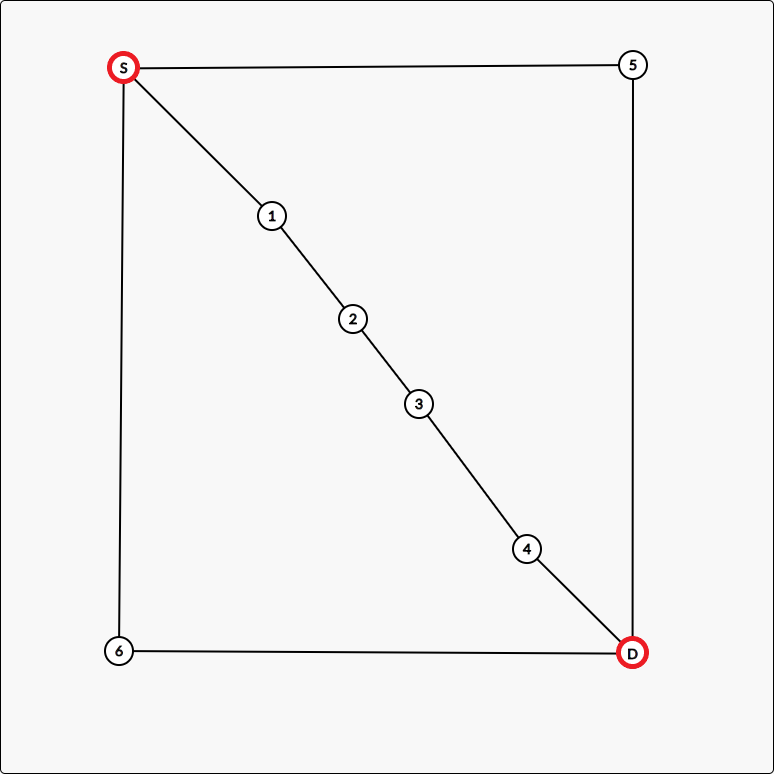
\includegraphics[scale=0.5]{problem_04.png} \\
    Рис. 5
\end{center}

Очевидно, кратчайший путь - это $S-1-2-3-4-D$. Припустим, что исполняющий алгоритм достиг вершины $2$ и в этот момент на ребре $2-3$ что-то случается, его перекрывают или там возникает беспросветная \glqq пробка\grqq, а короткого объезда нет, только возврат и движение по путям $S-5-D$ или $S-6-D$. Помимо таких сценариев, это ещё и частный случай проблемы 1), когда пути $S-5-D$ или $S-6-D$ могут быть заранее более выгодными, чем самый короткий по расстоянию.

Однако, можно предпринять определённые шаги, которые помогут избежать проблемы таких \glqq узких\grqq \ мест. Достаточно убрать такое ребро из графа и высчитать альтернативный путь. Не составит труда подсчитать его \textit{временную} сложность и сравнить с исходной сложность самого короткого пути \textit{по расстоянию}, и выбрать среди них лучший. 

Последний не решённый вопрос - как именно определять такие проблемные рёбра? Ничего сложного тут тоже нет, поскольку можно заранее найти все \glqq узкие\grqq \ места во всём графе $G_T$. Перебираем каждое ребро $e(u,v) \in E$ по очереди. Для каждой пары вершин $u$ и $v$ удаляем из графа ребро $e(u,v)$ и считаем наименьшее расстояние от вершины $u$ до вершины $v$. Если оно больше наперёд заданной константы $L_{narrow}$, тогда объезд этого ребра слишком длинный и это ребро является \glqq узким\grqq местом, помечаем его и переходим к оставшимся ещё не рассмотреным рёбрам. Таким образом, получим множество всех потенциально проблемных рёбер $V_{narrow}$.  

\subsection{Описание}

Алгоритм поиска кратчайшего пути \textit{по времени} в окрестности кратчайшего пути \textit{по расстоянию}: \\
\textbf{Шаг 1.} Высчитываем кратчайший путь $P^\prime(s,d)$ \textit{по расстоянию}. Получаем для него $L_t(P^\prime(s,d))$\\
\textbf{Шаг 2.} Для каждого ребра $v_i \in V_{narrow}: v_i \in P$ высчитываем \textit{альтернативный} кратчайший путь \textit{по расстоянию} $P_i^{\prime\prime}(s,d)$ и его временную стоимость $L_t(P_i^{\prime\prime}(s,d))$. Выбираем такой путь $P(s,d)$, что $L_t(P(s,d)) = \min_t\{L_t(P^\prime(s,d)), L_t(P_i^{\prime\prime}(s,d))\}$ $ \forall i$ \\
\textbf{Шаг 3.} Для наперёд заданной константы $T_{max}$ разбиваем путь $P(s,d)$ на $n$ подпутей $P(u_i,v_i)$, так что $P(s,d) = \bigcup\limits_{i=1}^{n}P(u_i,v_i),$  $L_t(P(u_i,v_i)) \leq T_{max}$ и $n$ минимально. \\
\textbf{Шаг 4.} Для каждого подпути $P(u_i,v_i)$ высчитываем самый короткий путь $P^*(u_i,v_i)$ \textit{по времени} в \textit{редуцированном} подграфе $G_{T,i} \subseteq   G_T$, содержащем $P(u_i,v_i)$. $G_{T,i}$ получается из графа $G_T$ взятием всех тех его вершин, находящихся на расстоянии меньше $R_{max}$ от любой точки на подпути $P(u_i,v_i)$.\\
\textbf{Шаг 5.} Объединяем полученные решения и получаем результат: $P(s,d) = \bigcup\limits_{i=1}^{n}P^*(u_i,v_i),$

\section{Реализация}

В качестве алгоритма поиска кратчайшего пути \textit{по расстоянию} используется алгоритм Дейкстры в виду простоты реализации и небольшого размера графа. Для больших же графов предполагается к использованию намного более эффективный алгоритм NBA* \cite{nba} с 4-5 кратным приростом скорости.

В качестве алгоритма поиска кратчайшего пути \textit{по времени} используется модифицированный алгоритм Дейкстры, который от оригинала отличается тем, что в качестве меток для вершин берётся время, затрачиваемое на путь к ним от начальной вершины. Также, функция подсчёта веса ребра принимает ещё и временной параметр, на основании которого определяется скорость движения на ребре: 
$$weight(e, t) = l(e) / v_{act}(e, t)$$

\begin{algorithm}
\caption{Modified Dijkstra's algorithm}
\begin{algorithmic}[1]

\State \textbf{for} each vertex $v \in \id{V_G}$ \\
    \qquad $\at{cost}[v] \gets \infty$ \\
    \qquad $\at{parent}[v] \gets \const{NIL}$ \\
$\at{cost}[s] \gets 0$ \\
\\
$Q \gets \id{V_G}$
\State \textbf{while} $Q \neq \emptyset$ \\
\qquad $u \gets \text{Extract-Min}(Q)$ \\
\qquad \textbf{for} each edge $e = (u,v)$ \\
\qquad \qquad \textbf{if} $\at{cost}[v] > \at{cost}[u] + \at{weight}(e, t_0 + cost[u])$ \\
\qquad \qquad \qquad $\at{cost}[v] \gets \at{cost}[u] + \at{weight}(e, t_0 + cost[u])$ \\
\qquad \qquad \qquad $\at{parent}[v] \gets u$ \\
\\
$H \gets (\id{V_G, \emptyset})$
\State \textbf{for} each vertex $v \in \id{V_G},\ v \neq s$ \\
    \qquad $\id{E_H} \gets \id{E_H} \cup \{(\at{parent}[v], v)\}$ \\
\Return $H, \id{cost}$
\end{algorithmic}
\end{algorithm}

\pagebreak
\section{Результаты}

Была сделана программная реализация предложенного алгоритма (и сопутствующих ему компонентов), позволяющая:

\begin{itemize}
    \item визуализировать заданный граф, весы рёбер и пути на нём 
    \item находить множество рёбер $V_{narrow}$
    \item редуцировать граф до окрестности заданного пути
    \item вычислять кратчайшие пути \textit{по расстоянию} и \textit{по времени}
\end{itemize}

В качестве графа для тестирования использовался сгенерированный граф из 100 вершин и 167 рёбер. Весы рёбер, представляющие среднюю скорость движения на ребре, в основном задавались случайно сгенерированными величинами (некоторым рёбрам скорость движения была выставлена вручную для имитации \glqq пробок\grqq \ в \glqq узких\grqq \ местах графа). 

Несколько характерных примеров работы алгоритма показаны на Рис. 6а и Рис. 6б. Жёлтым изображены кратчайшие пути \textit{по расстоянию}, зелёным - \textit{по времени}. В первом случае алгоритм находит более быстрые альтернативы для участков пути. Во втором же предлагает полностью другой обходной путь из-за низкой скорости движения на \glqq мосту\grqq \ (ребре в центре пути, который соединяет два компонента связности, и является \glqq узким\grqq \ местом для графа).

Тестируемый граф в виду своих небольших размеров не позволил найти ответа на вопрос выбора оптимального параметра $R_{max}$, поскольку даже при выборе $R_{max} = \infty$ заметной разницы в скорости работы алгоритма не было замечено. Следовательно, единственное, что можно уверенно заявить - следует выбирать такой $R_{max}$, который в среднем при редукции графа в области пути продолжительностью меньше $T_{max}$ давал подграф $G=(V,E)$ размерности $N(G) = |V| + |E|$ , где $N$ не меньше, чем у заданного графа ($N(G_{test}) = 267$).
 
\begin{figure}
\minipage{0.5\textwidth}
  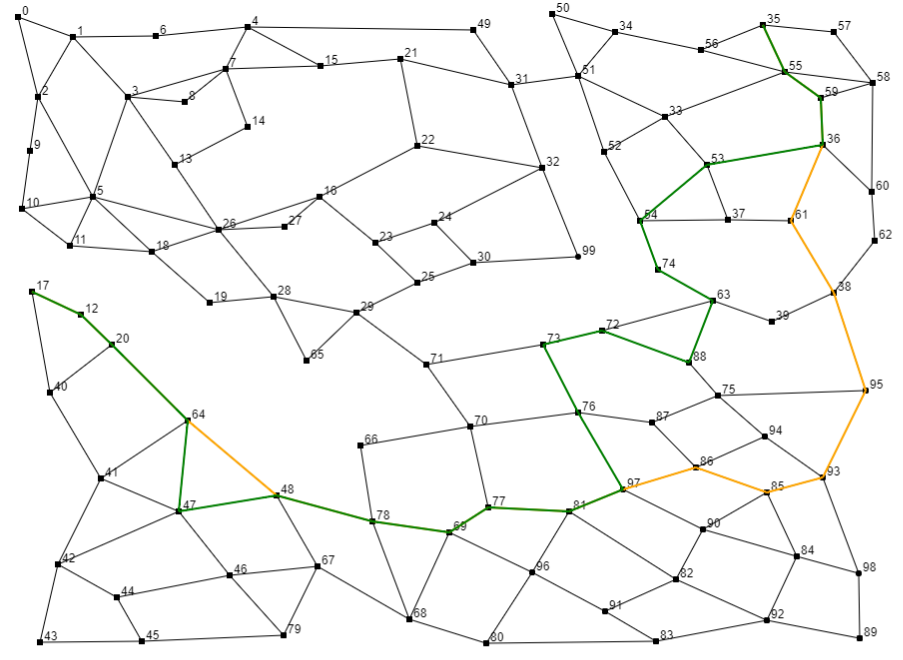
\includegraphics[width=\linewidth]{result_01.png}
    \begin{center}
        Рис. 6а
    \end{center}
\endminipage\hfill
\minipage{0.5\textwidth}
  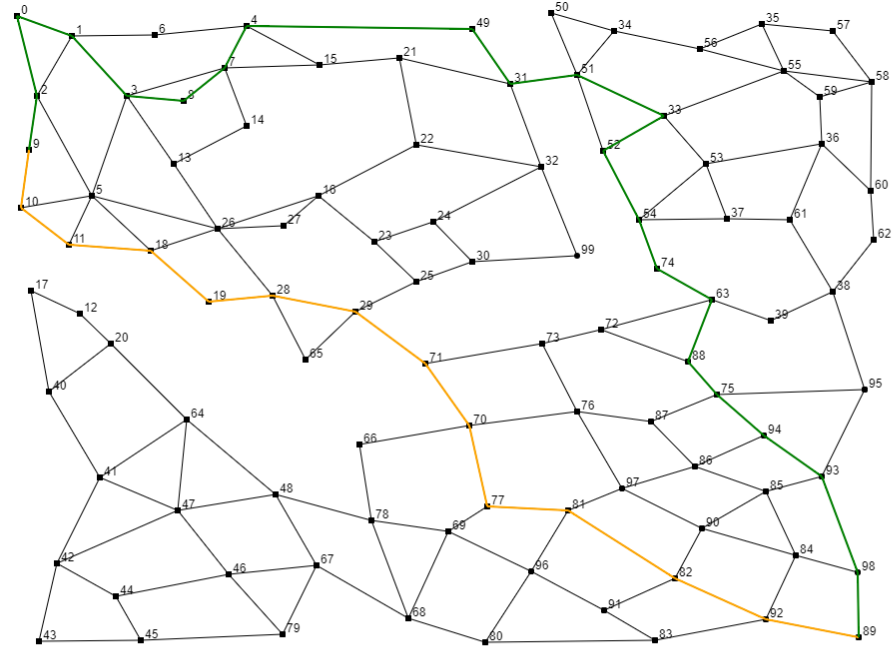
\includegraphics[width=\linewidth]{result_02.png}
        \begin{center}
        Рис. 6б
    \end{center}
\endminipage
\end{figure}

\pagebreak
\begin{thebibliography}{}
    \bibitem{vics} Vehicle Information and Communication System. http://www.vics.or.jp/en/
    \bibitem{tmc} Traffic Message Channel. https://en.wikipedia.org/wiki/Traffic\_message\_channel
    \bibitem{survey} Amgad Madkour, Walid G. Aref, Faizan Ur Rehman, Mohamed Abdur Rahman, Saleh
Basalamah. A Survey of Shortest-Path Algorithms. Purdue University, West Lafayette, USA.
Umm Al-Qura University, Makkah, KSA. May 8, 2017
    \bibitem{2s-ltt} B. Ding, J. X. Yu, and L. Qin. Finding time-dependent shortest paths over large graphs.
Proceedings of the 11th international conference on Extending database technology Advances
in database technology EDBT 08, page 205, 2008.
    \bibitem{or} A. Orda and R. Rom. Shortest-path and minimum-delay algorithms in networks with time-dependent edge-length. J. ACM, 37(3):607–625, 1990.
    \bibitem{kdxz} E. Kanoulas, Y. Du, T. Xia, and D. Zhang. Finding fastest paths on a road network with speed patterns. In ICDE, pages
10–19, 2006.
    \bibitem{dot}  I. Chabini. Discrete dynamic shortest path problems in transportation applications: Complexity and algorithms with optimal run time. Transportation Research Record,
1645:170–175, 1998.
    \bibitem{tiger} Topologically Integrated Geographic Encoding and Referencing system: http://www.census.gov/geo/www/tiger/
    \bibitem{nba} Wim Pijls, Henk Post. Yet another bidirectional algorithm for shortest paths. Econometric Institute Report EI 2009-10. 15 June, 2009
\end{thebibliography} 

\end{document}
